\documentclass[12pt,pscyr]{hedlab}
\usepackage[russian]{babel}
\usepackage{graphicx}
\graphicspath{{images/}}

\labname{Автоматизация торгового предприятия при помощи 1С\\Вариант 42}
\labnum{4}
\student{Чечеткин И. А., САПР-1.1п}
\labdate{}

\begin{document}

  \makeheader
  \emph{Задание:}
  Компания является заведением общественного питания. Возможна продажа как
  отдельных продуктов, так наборов этих продуктов и готовых блюд.
  
  Набор представляет из себя перечень продуктов, хранящихся на складе.
  Например, можно продавать в виде набора пирожное и чай, а можно по
  отдельности~-- отдельно чай, отдельно пирожное. В том случае, если из
  продуктов изготовлено блюдо, например из овощей сделан салат, то продаваться
  может только само блюдо, а входящие в его состав продукты проданы быть не
  могут.
  
  Закупка продуктов отражается документом <<Приходная накладная>>,
  продажа~-- <<Расходная накладная>>. Для отражения приготовления блюд и
  создания наборов служит документ <<Комплектация>>. Учет остатков в разрезе
  складов не ведется.
  
  При продаже в одной табличной части указываются продукты, наборы и готовые
  блюда. В документе <<Комплектация>> в табличной части указывается продукты и
  их количество, а в шапке набор или готовое блюдо и его количество. В состав
  набора и готового блюда могут входить как продукты, так и готовые блюда. В
  случае приготовления блюда, должно произойти списание необходимого количества
  продуктов и оприходование готовых блюд в количестве, указанном в шапке
  документа. В случае комплектации набора, при продаже необходимо будет списать
  столько продуктов, сколько их входит в набор.
  
  Со временем (не чаще, чем 1 раз в день) состав набора может изменяться, для
  чего необходимо создать новую комплектацию этого набора. Создавать набор или
  вносить изменения в него можно только документом <<Комплектация>>. При продаже
  должен приниматься тот состав набора, который был актуальным на момент
  продажи.
  
  Себестоимость при списании рассчитывается как средняя.
  
  Необходимо создать отчеты о движении складских запасов и о продажах за
  период.\\
  
  \emph{Скриншоты}
  \begin{figure}[h!]
    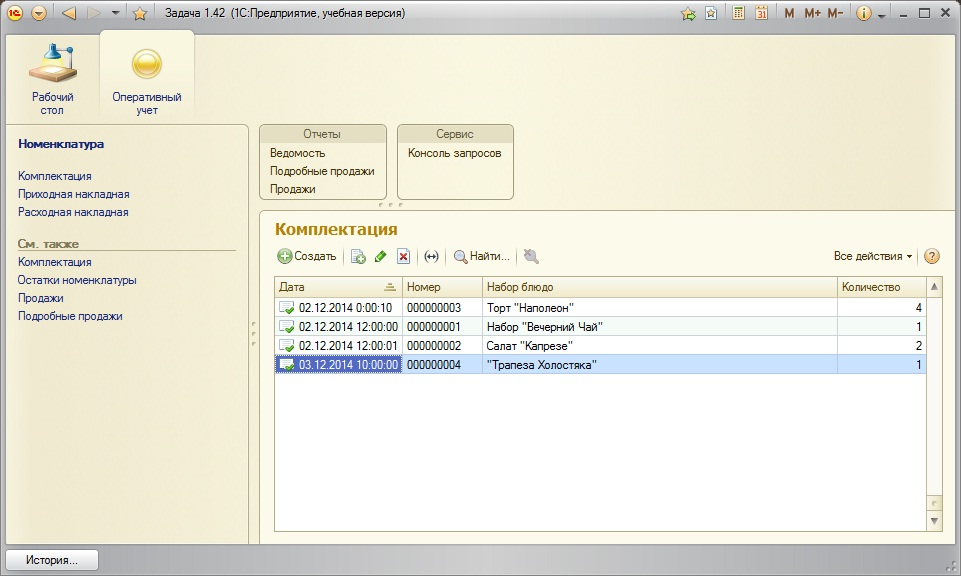
\includegraphics[width=.5\textwidth]{1c_1}
    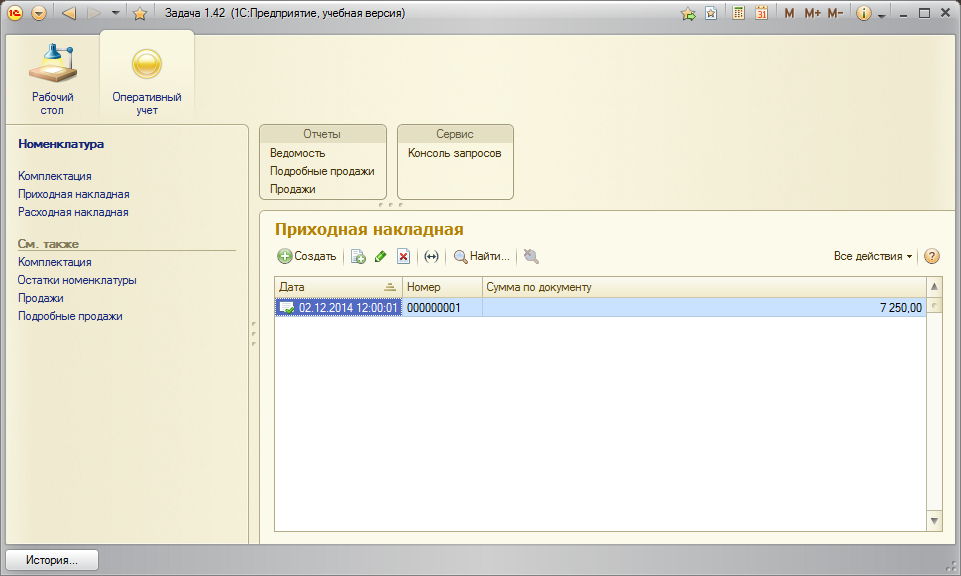
\includegraphics[width=.5\textwidth]{1c_2}\\
    \parbox{.5\textwidth}{\caption{Документ <<Комплектация>>}}
    \parbox{.5\textwidth}{\caption{Документ <<Приходная накладная>>}}
  \end{figure}
  
  \pagebreak
  
  \begin{figure}[h!]
    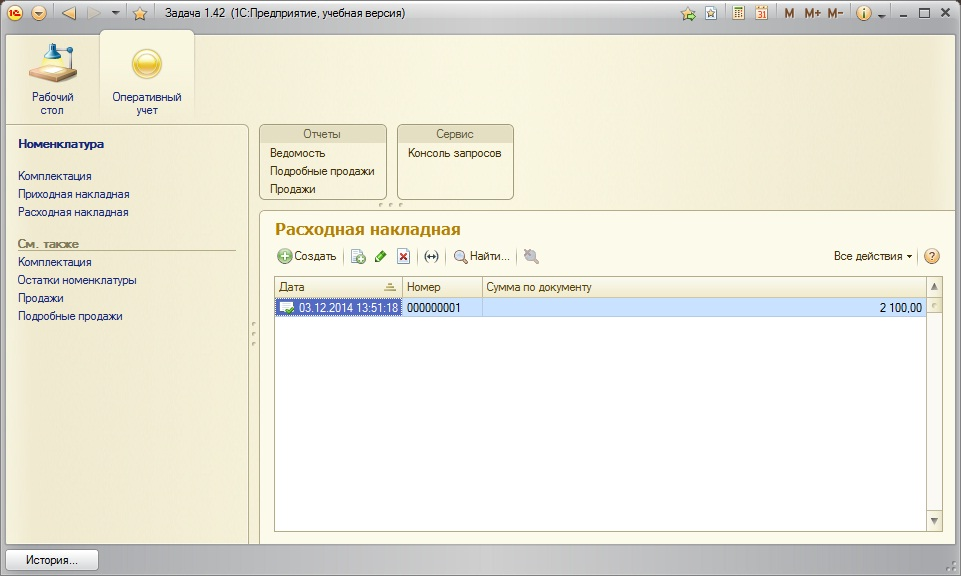
\includegraphics[width=.5\textwidth]{1c_3}
    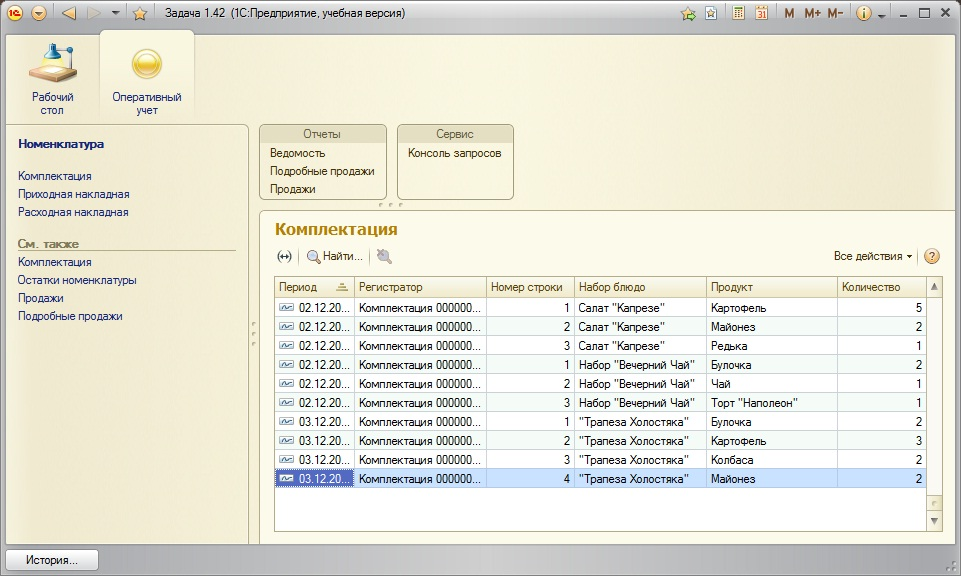
\includegraphics[width=.5\textwidth]{1c_4}\\
    \parbox{.5\textwidth}{\caption{Документ <<Расходная накладная>>}}
    \parbox{.5\textwidth}{\caption{Комплектация за период}}
  \end{figure}
  
  \begin{figure}[h!]
    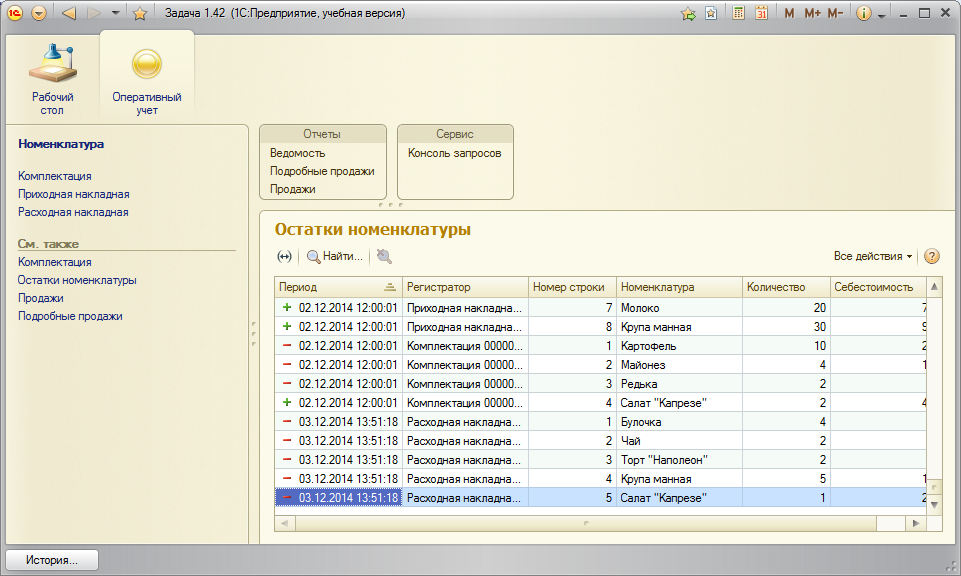
\includegraphics[width=.5\textwidth]{1c_5}
    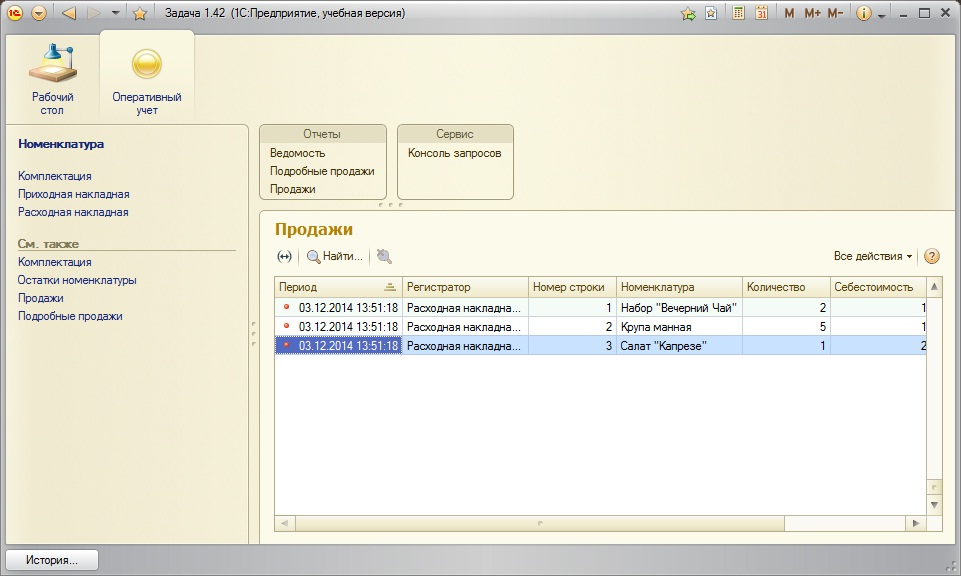
\includegraphics[width=.5\textwidth]{1c_6}\\
    \parbox{.5\textwidth}{\caption{Остатки номенклатуры}}
    \parbox{.5\textwidth}{\caption{Продажи за период}}
  \end{figure}
  
  \begin{figure}[h!]
    \center
    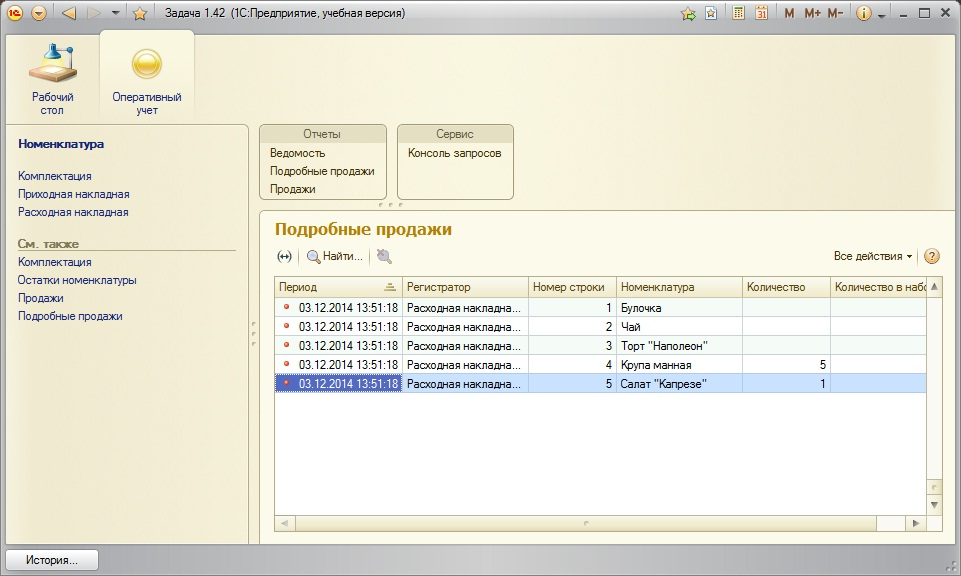
\includegraphics[width=.5\textwidth]{1c_7} \\
    \parbox{.5\textwidth}{\caption{Подробные продажи}}
  \end{figure}
 
  \emph{Вывод:} в ходе лабораторной работы были получены навыки работы с
  программной системой 1С Предприятие.

\end{document}